% !TeX TS-program = txs:///duck
\documentclass{standalone}
\usepackage{tikzducks,tikzlings}

\usetikzlibrary{decorations.shapes,shapes.geometric} \tikzset{
  paint/.style={draw=#1, fill=#1},
  decorate with/.style={
    decorate,
    decoration={shape backgrounds,shape=#1,shape size=2mm}
  }
}

\begin{document}
	
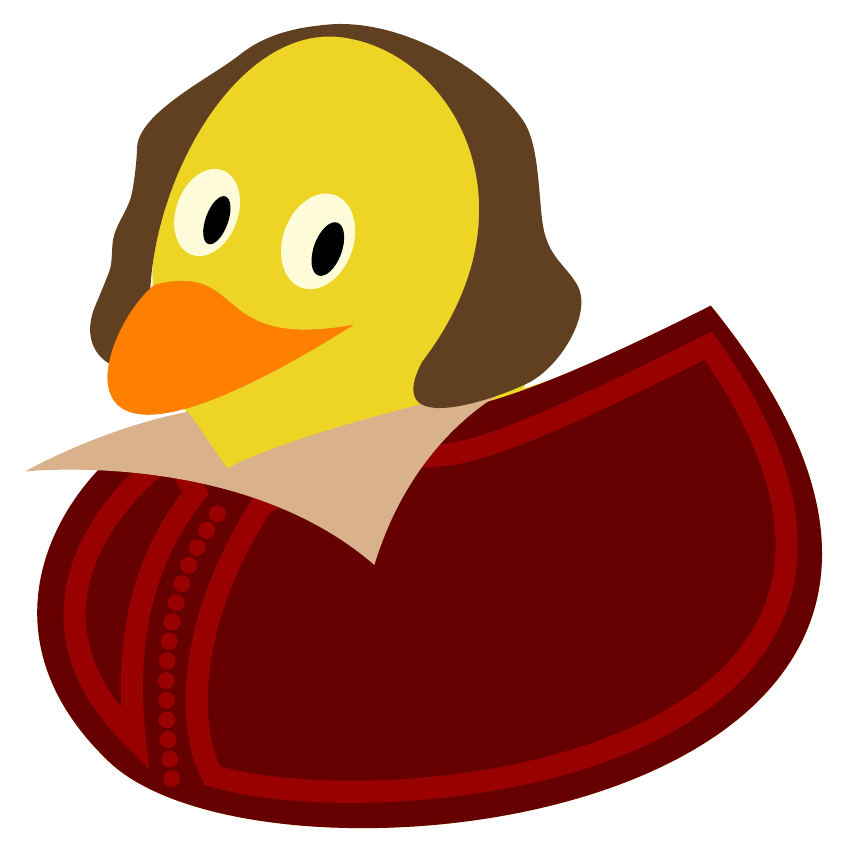
\begin{tikzpicture}[scale=5]
	\duck[tshirt=red!40!black]
  
  \begin{pgfinterruptboundingbox}
    
    % decorative lines 
    \draw[red!60!black, line width=8pt] (0.4516,1.0436) .. controls (0.3563,0.9851) and (0.0028,0.6638) .. (0.3551,0.3180) .. controls (0.3176,0.6584) and (0.4305,0.8439) .. (0.5095,0.9433) -- cycle;
    \draw[red!60!black, line width=8pt] (0.5528,0.2249) .. controls (1.0301,0.0845) and (2.5509,0.2722) .. (1.8114,1.3178) .. controls (0.8728,0.8445) and (1.3067,1.1798) .. (0.6800,0.9162) .. controls (0.4872,0.6211) and (0.4847,0.3481) .. (0.5528,0.2249) -- cycle;
    
    % buttons
    \draw[decorate with=circle, paint=red!60!black] (0.4488,0.2173) .. controls (0.4113,0.5578) and (0.4478,0.7328) .. (0.5858,0.9190);
    
    % collar
    \fill[brown!60!white] (0.4903,1.1495) .. controls (0.2672,1.1065) and (0.0760,0.9976) .. (0.0760,0.9976) .. controls (0.0760,0.9976) and (0.6221,1.0565) .. (0.9635,0.7604) .. controls (1.0802,1.1411) and (1.3613,1.2348) .. (1.3613,1.2348) .. controls (0.7249,1.0939) and (0.5904,1.0045) .. (0.5904,1.0045) -- cycle;
  
    % hair
    \fill[brown!50!black] (1.3513, 1.2210) .. controls (1.436, 1.2619) and (1.5207, 1.4022) .. (1.4779, 1.4733) .. controls (1.4478, 1.5233) and (1.404, 1.5447) .. (1.3918, 1.6228) .. controls (1.3795, 1.7009) and (1.3832, 1.8319) .. (1.3396, 1.8918) .. controls (1.2345, 2.0363) and (1.0169, 2.1484) .. (0.8458, 2.1329) .. controls (0.7602, 2.1251) and (0.6856, 2.1076) .. (0.6193, 2.0544) .. controls (0.553, 2.0013) and (0.3646, 1.9095) .. (0.361, 1.821) .. controls (0.3594, 1.7811) and (0.3548, 1.7426) .. (0.3481, 1.7058) .. controls (0.3414, 1.6689) and (0.3132, 1.6336) .. (0.3031, 1.6000) .. controls (0.2931, 1.5664) and (0.3012, 1.5344) .. (0.2896, 1.5041) .. controls (0.278, 1.4739) and (0.2661, 1.4453) .. (0.2547, 1.4186) .. controls (0.2068, 1.3059) and (0.2969, 1.2225) .. (0.4156, 1.2723) .. controls (0.3158, 1.5798) and (0.5698, 2.1437) .. (0.8839, 2.1002) .. controls (1.1639, 2.0615) and (1.3879, 1.672) .. (1.0851, 1.2765) .. controls (0.9804, 1.0784) and (1.2697, 1.1816) .. (1.3513, 1.2210) -- cycle;
  
    % redraw bill on top of the hair
    \fill[orange] \duckpathbill;
  
  \end{pgfinterruptboundingbox}

\end{tikzpicture}	
	
\end{document}